\chapter{Experiment}
\label{ch:experiment}

\newcommand{\takeaway}[1]{
\vspace{6pt}
\noindent\fbox{\parbox{\textwidth}{#1}}
\vspace{6pt}
}
We would like to evaluate the cost of computing one single IVC using the brute-force
algorithm (\ucbfalg) and the UNSAT core-based algorithm (\ucalg).
Then, we are interested in examining the {\em efficacy} and {\em efficiency} of generating all minimal IVCs, as compared to algorithms for computing a {\em single approximately minimal} IVC (\ucalg\ algorithm), and a {\em minimal IVC} (\ucbfalg\ algorithm).  We would also like to know how performance is affected by the size of models and number of minimal IVCs.  Next, we are also interested in examining the minimality of the cores found by \ucbfalg\ vs  \ucalg . Finally we would like to determine whether the \aivcalg\ algorithm generates {\em smaller} cores than are generated by the \ucbfalg\ algorithm.  %If the AIVC algorithm is similarly efficient to \ucbfalg\ then several analyses can be performed that would not be possible with a single \mivc\computed from the \ucbfalg\ algorithm.
%
%
Therefore, we investigate the following research questions:
\begin{itemize}
  \item \textbf{RQ1:} How expensive is it to compute IVCs?  For this question we examine the cost of the \ucalg ~and \ucbfalg ~algorithms that find a single approximately minimal and guaranteed minimal IVC,respectively, as well as the \aivcalg ~algorithm for determining all minimal IVCs.
  \item \textbf{RQ2:} How is the verification time of the \aivcalg ~algorithm affected by the baseline proof time and the number of IVCs that can be found for a property?
   \item \textbf{RQ3:} How close to minimal are the IVCs computed by \ucalg\ as opposed to the (guaranteed minimal) \ucbfalg\ and the \emph{minimum} IVC computed by \aivcalg ?  How do the sizes of IVCs compare to static slices of the model?
 % \item \textbf{RQ4:} How large are the IVCs produced by the \aivcalg\ algorithm
  %  compared to those of \ucalg\ and \ucbfalg ?
%
%  \item \textbf{RQ3)} How does approximating minimality influence the performance of the \aivcalg ~algorithm?
%  In other words, we would like to determine, for the implementation of the \getivc ~procedure, whether it would be better to use \ucalg ~or \ucbfalg .
%  \item \textbf{RQ4)} How did the pre-set timeout manifest itself in the experimental results?
\end{itemize}


\subsection{Experimental Setup}

Our experiments are conducted on a set of benchmarks containing 660 Lustre models, including all of the benchmark models yielding a valid result (530 in total) from~\cite{Hagen08:FMCAD, piskac2016} and 130 industrial models yielding valid results derived from an infusion pump system \cite{hilt2013} and other sources \cite{piskac2016, NFM2015:backes}.
Most of the academic benchmark models are small (10kB or less, with 6-40 equations) and include a range of hardware benchmarks and software problems involving counters that are difficult to solve inductively.
The industrial models are much larger; for example, each of the 80 problems from the infusion pump \cite{hilt2013} contain over 600 equations and are each $\geq$80kB in size. The benchmark includes 2 models from the NASA Quad-redundant Flight Control System (QFCS)~\cite{NFM2015:backes}: the Flight Control System (FCS) with 5259 Lustre equations and the Flight Control Computer (FCC) with 10969 equations.

We selected only benchmark problems consisting of a Lustre model with
properties that \texttt{JKind} could prove with a 3-hour timeout.
For each test model, we computed \aivcalg, \ucalg, and \ucbfalg ~algorithms in a configuration with the \texttt{Z3} solver and the ``fastest'' mode of \texttt{JKind} (which involves running the $k$-induction and PDR engines in parallel and terminating when a solution is found). The experiments were run on an  Intel(R) i5-4690, 3.50GHz, 16 GB memory machine running Linux, and are available online~\cite{expr}.%\footnote{The benchmarks, tools, and experimental results are available on \cite{expr}.}



\subsection{Experimental Results}

\section{Results}
\label{sec:results}

\newcommand{\takeaway}[1]{
\vspace{6pt}
\noindent\fbox{\parbox{\columnwidth}{#1}}
\vspace{6pt}
}

In this section, we examine our experimental results from three perspectives: performance, minimality of \ucalg results and diversity.

\iffalse
\mike{Results and Discussion:}
\begin{itemize}
    \item (Overview) Give an overview of results, possibly referencing a graph or two.
    \item Statistical analysis: provide positive and null hypotheses for the research questions.
    \item Evaluation of research questions: statistical results and explanations of the graphs.  One subsection per research question?
    \item Threats to validity: what are our threats?
    Internal validity: not really necessary, I think.
    External validity (how much can the results be generalized):
        1. currently all models are *very small*;
        2. Many programs were drawn from mutations of a relatively small number of ``seed'' programs;
        3. The models are written in Lustre rather than FOL.  This means that the
            top-level conjunctions are all over equations rather than general
            form;
        4. Others?!?
    Construct validity: we are measuring what we think we're measuring: IVC and minimality are reasonably defined.  For discussions of ``completeness'' and ``traceability'' we need to be clear about any claims (probably not in this paper).
\end{itemize}
\fi

\subsection{Performance}
\label{sec:performance}

In this subsection, we examine the performance of our inductive validity core algorithms (research question \textbf{RQ1}).  First we examine the performance overhead of the \ucalg algorithm over the time necessary to find a proof using inductive model checking.  To examine this question, we use the default {\em fastest} option of JKind which terminates when either the k-induction or PDR algorithm finds a proof.  To measure the performance overhead of the \ucalg algorithm, we execute it over the proof generated by the {\em fastest} option.

Since the \ucalg algorithm uses the UNSAT-core facilities of the underlying SMT solver, the performance is dependent on the efficiency of this part of the solver.  Examining Tables~\ref{tab:runtime-ucalg} and~\ref{tab:overhead-ucalg}, it is possible to examine both the aggregate computation time for analysis using the four solvers under evaluation and the overhead imposed by the \ucalg algorithm.  The data suggests that yices (the default solver in JKind) and z3 are the most performant solvers both in terms of computation time and overhead.  Figure~\ref{fig:runtimeall} allows a visualization of the overhead for the \ucalg algorithm running different tools (as well as the \bfalg, discussed below).  For this figure, models are ranked on the x-axis in terms of their analysis time using the z3 solver to perform the proof without performing IVC.

%Figure~\ref{fig:runtimez3} allows a visualization of the overhead for the Z3 solver, where the models are ranked on the x axis in terms of their analysis time without performing \ucalg, and the y-axis describes analysis time with and without \ucalg.

%\mike{Add the raw timings for each solver for proof and proof + \ucalg analysis in Table~\ref{tab:overhead}.}

%Although it is relatively obvious from Table~\ref{tab:overhead}, it is straightforward to demonstrate with statistical significance that Z3 outperforms other solvers.  The hypotheses are as follows: \mike{FILL IN HYPOTHESES}.

%\mike{Do we need hypotheses here?  We could say a 'moderate' performance penalty is under 50\% over the regular solver time}.

\takeaway{The \ucalg algorithm using the Z3 and yices SMT solvers adds a modest performance penalty to the time required for inductive proofs.}

Next, we consider the overhead of \ucalg vs. \bfalg.  Recall from Section~\ref{sec:ivc} that \bfalg requires $n$ model checking runs, where $n$ is the number of conjuncts in the transition relation. As expected, the performance is approximately a linear multiple of the size of the model, so larger models yield substantially lower performance.\footnote{for Lustre models, the number of conjuncts is equivalent to the number of equations in the Lustre model.}  We run the brute-force algorithm using yices as it is the default solver for JKind and is close to z3 in terms of computation time.  For 19 models, \bfalg times out after 1 hour.   Figure~\ref{fig:runtimeall} shows the overhead of \bfalg in comparison to \ucalg with multiple solvers.

\takeaway{The brute-force algorithm \bfalg adds a substantial performance penalty to inductive proofs in all cases and is not scalable enough to compute a minimal core for large analysis problems.}

Finally, we consider the combined \ucbfalg algorithm, in which we first run the \ucalg to determine a close-to-minimal set of support, then run the \bfalg on the remaining set.  The overhead of this algorithm is considered in Tables~\ref{tab:runtime-ucbfalg} and~\ref{tab:overhead-ucbfalg}.  While considerably slower than the \ucalg, this approach can still be used for reasonably sized models.

\begin{figure*}
  \centering
  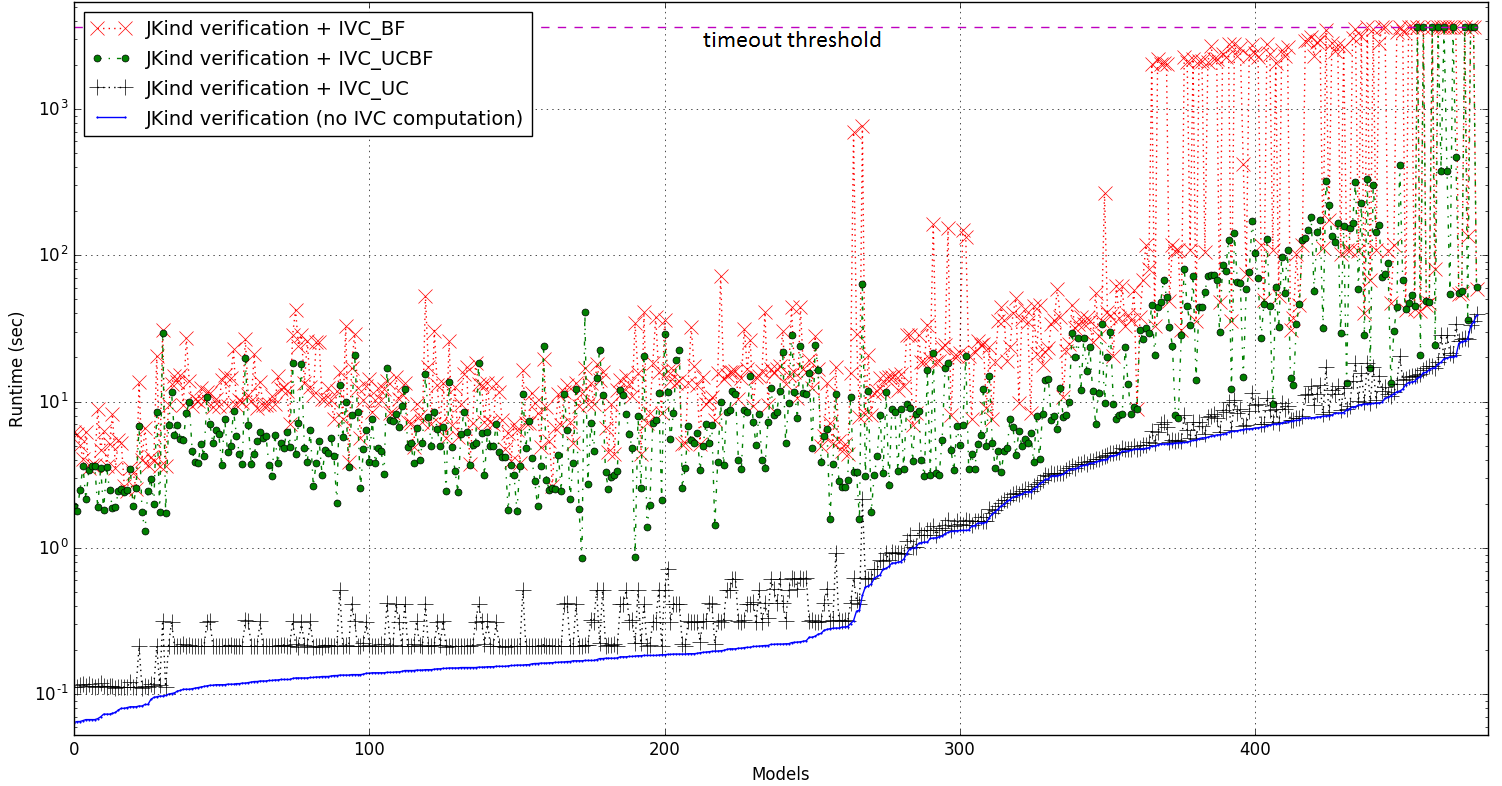
\includegraphics[width=\textwidth]{figs/timing_analyses.png}
  \vspace{-0.3in}
  \caption{Runtime of \bfalg, \ucbfalg, \ucalg algorithms for Yices}\label{fig:runtimeall}
\end{figure*}

%\vspace{-0.5in}
\begin{figure*}
  \centering
  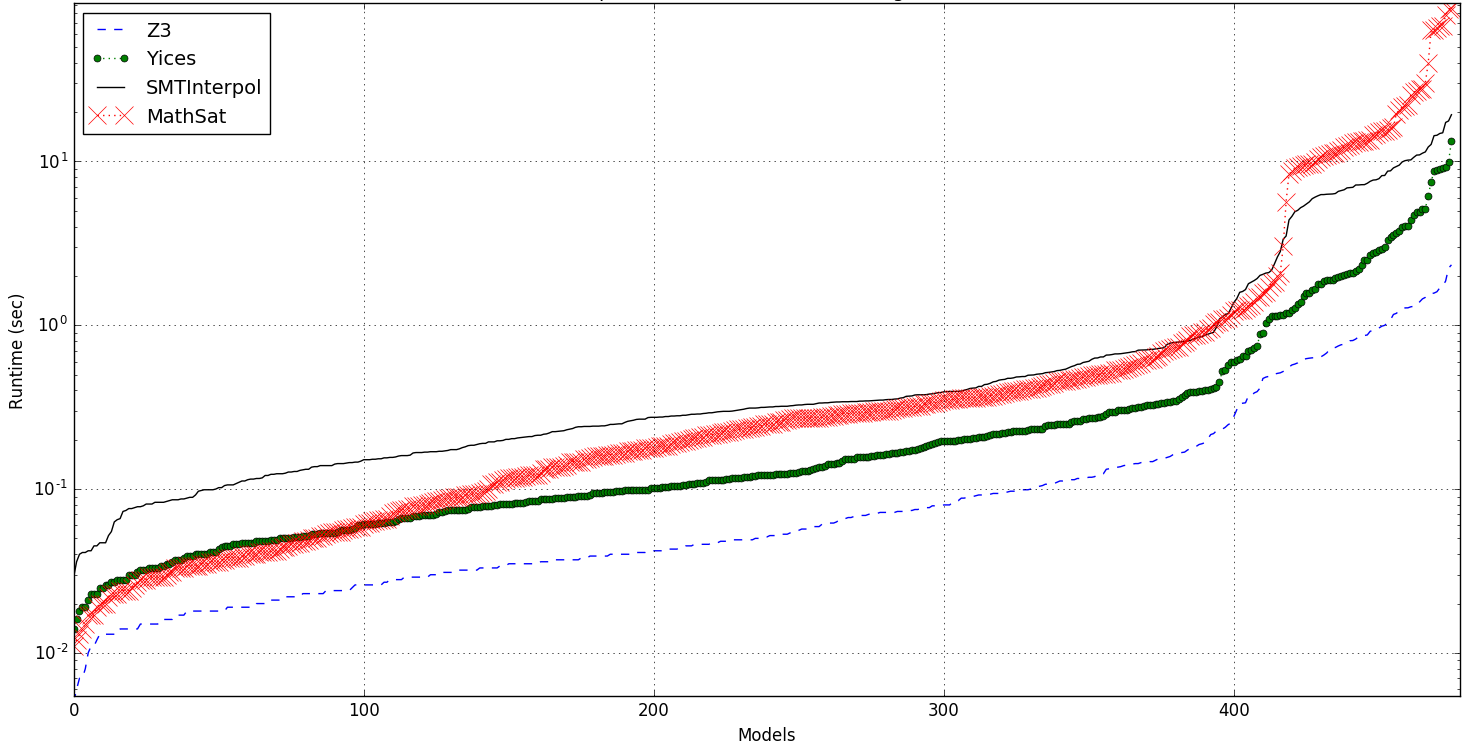
\includegraphics[width=\textwidth]{figs/performance.png}
  \vspace{-0.3in}
  \caption{\ucalg performance on different solvers}\label{fig:performance}
\end{figure*}

\begin{table}
  \centering
  \begin{tabular}{ |c||c|c|c|c| }
    \hline
     runtime (sec) & min & max & mean & stdev \\[0.5ex]
    \hline\hline
 %   JSupport & 2.381 & 165.157 & 21.533 & 23.533 \\[0.5ex]
    Z3   & 0.005 & 2.335 & 0.192 & 0.355 \\[0.5ex]
    Yices &   0.014  & 13.297   & 0.589 & 1.473 \\[0.5ex]
    SMTInterpol& 0.029 & 19.254 &  1.396 & 2.991 \\[0.5ex]
    MathSAT & 0.011 & 86.421 &  3.071 & 10.403 \\[0.5ex]
    \hline
  \end{tabular} \\
  \caption{\ucalg runtime with different solvers}
  \label{tab:runtime-ucalg}
\end{table}

\begin{table}
  \centering
  \begin{tabular}{ |c||c|c|c|c| }
    \hline
     solver & min & max & mean & stdev \\[0.5ex]
    \hline
    Z3   & 0.73\% & 84.13\% & 17.38\% & 16.92\% \\[0.5ex]
    Yices &   0.17\%  & 351.47\%   & 52.20\% & 54.50\% \\[0.5ex]
    SMTInterpol& 1.46\% & 175.75\% &  46.81\% & 37.35\%\\[0.5ex]
    MathSAT & 0.78\% & 955.52\% &  80.21\% & 112.92\%\\[0.5ex]
    \hline
  \end{tabular}
  \caption{Overhead of \ucalg computations using different solvers}
  \label{tab:overhead-ucalg}
\end{table}

\begin{table}
  \centering
  \begin{tabular}{ |c||c|c|c|c| }
    \hline
     runtime (sec) & min & max & mean & stdev \\[0.5ex]
    \hline
    Yices &   0.678  & 3600.0   & 91.594 & 490.008 \\[0.5ex]
    \hline
  \end{tabular}
  \caption{\ucbfalg runtime with Yices}
  \label{tab:runtime-ucbfalg}
\end{table}

\begin{table}
  \centering
  \begin{tabular}{ |c||c|c|c|c| }
    \hline
     solver & min & max & mean & stdev \\[0.5ex]
    \hline
    Yices & 122.50\%  & 30092.78\%   & 3195.90\% & 3896.05\% \\[0.5ex]
    \hline
  \end{tabular}
  \caption{Overhead of \ucbfalg algorithm using Yices}
  \label{tab:overhead-ucbfalg}
\end{table}
% over = in

\begin{table}
  \centering
  \begin{tabular}{ |c|c|c|c| }
    \hline
     solver & PDR & k-induction & \textbf{total} \\
    \hline
      z3 & 2378 & 2379 & 4757 \\
      yices & 2384 & 2376 & 4760 \\
      MathSAT & 2375 & 2369 & 4744 \\
      SMTInterpol & 2378 & 2368 & 4746 \\
    \hline
      \textbf{total} & 9515 & 9492 &   \\
    \hline
  \end{tabular}
  \caption{Aggregate IVC sizes produced by \ucalg\ using different inductive algorithms and solvers}
  \label{tab:minimality-algorithm-solvers}
\end{table}

\begin{table}
  \centering
  \begin{tabular}{ |c||c|c|c|c| }
    \hline
     solver & min & max & mean & stdev \\[0.5ex]
    \hline
    Yices &   0.0\%   & 7.25\% & 0.20\% & 0.50\% \\[0.5ex]
    \hline
  \end{tabular}
  \caption{Increase in IVC Size for \ucalg\ vs. \ucbfalg}
  \label{tab:overhead-ucbfalg}
\end{table}


\begin{figure*}
  \centering
  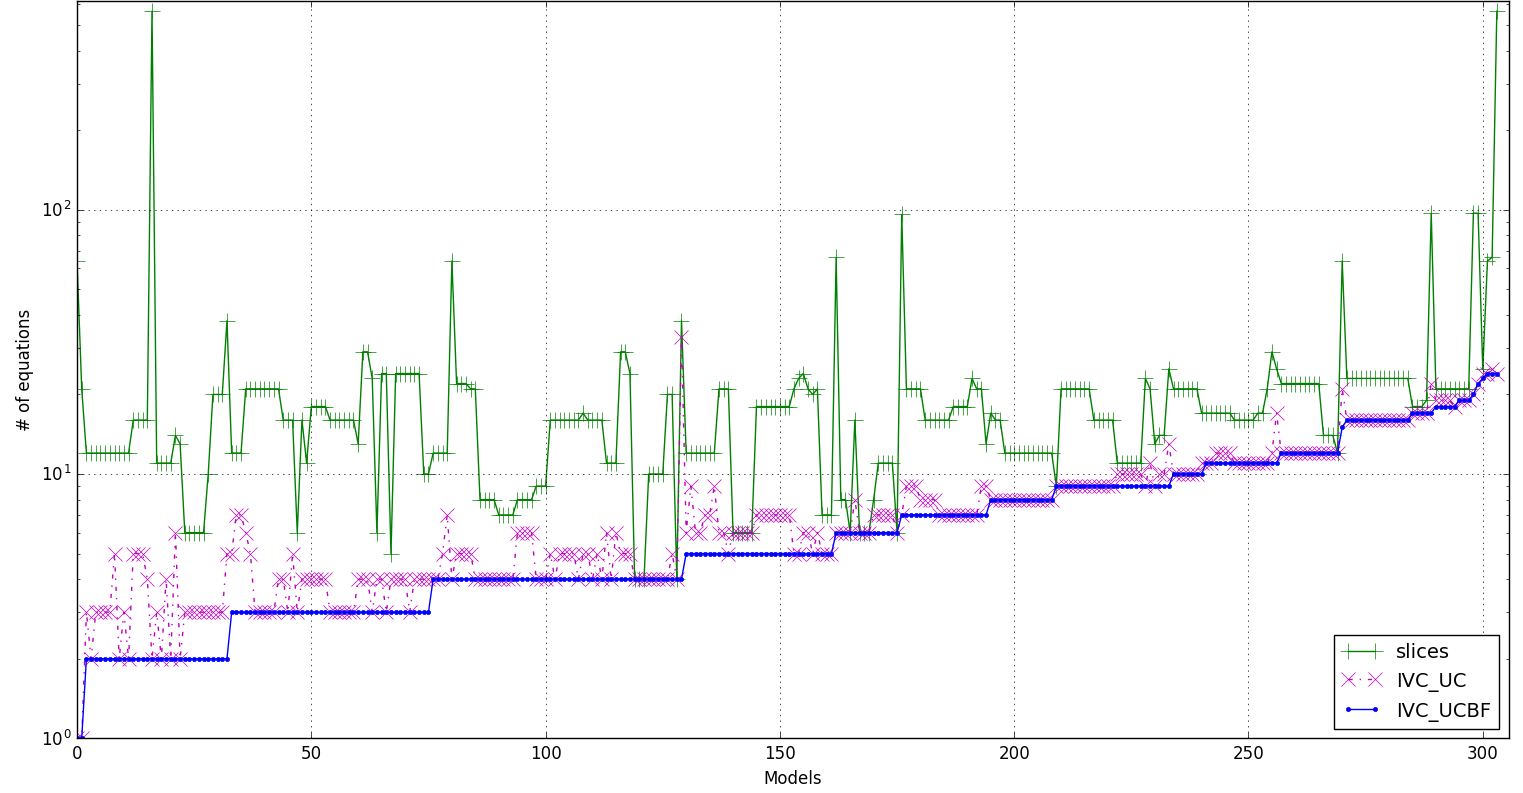
\includegraphics[width=\textwidth]{figs/minimality.png} 
  \caption{IVC sizes produced by \ucalg vs. \ucbfalg for Yices}
  \label{fig:minimality-all}
\end{figure*}

\subsection{Minimality}
\label{sec:minimality}
In this section, we examine the minimality of the cores computed by the \ucalg algorithm using different inductive proof methods and compare it to the cores produced by the combined algorithm (\textbf{RQ2}).  There are three interesting aspects to be examined related to this research question.  First (\textbf{RQ2.1}), does the choice of SMT solver or algorithm used to produce a proof (k-induction or PDR) matter in terms of the minimality of the inductive core?   As mentioned in Section~\ref{sec:ivc}, the \ucalg algorithm is not guaranteed to produce a minimal core due in part to the role of invariants used in producing a proof; as k-induction and PDR use different invariant generation algorithms, it is possible that one or the other is more likely to yield smaller invariant sets.  In addition, differences in the choice of the UNSAT-core algorithms in the different tools could affect the size of the generated core.  However, our algorithm {\em already} does a minimization step.  However,
our algorithm {\em already} does a minimization step on UNSAT-cores,
thus the only differences would be due to one algorithm leading to a
different minimal core than another.

As discussed in Section~\ref{sec:experiment}, k-induction is unable to solve all of the analysis problems; therefore we include only models that are solvable using {\em both} k-induction and PDR by {\em all tools}, 304 models in all.  Examining the aggregate data in Table~\ref{tab:minimality-algorithm-solvers}, we can see the sizes of cores produced by different algorithms and tools.

%if we sum all elements of all cores together, that PDR has an smaller core size in aggregate than k-induction.
%However, the data is noisy, and to examine \textbf{RQ2.1} systematically, we construct a hypothesis that PDR will, in general, equal or outperform k-induction on an arbitrary model:

%\mike{ADD HYPOTHESIS/NULL HYPOTHESIS HERE}

%Although the aggregate data suggests that PDR will yield a smaller core (on average) than k-induction, this claim is not supported for a given model with significance.

\takeaway{Neither PDR nor k-induction yields a smaller inductive validity core in general.}


%we already perform a linear scan of the cores generated by the SMT solver to remove unnecessary conjuncts

The next question (\textbf{RQ2.2}) asks how close to minimal are the cores produced by \ucalg\ vs. the (guaranteed minimal) cores produced by the \ucbfalg\ algorithm?  Note that we cannot measure the distance on all models because the combined algorithm times out on 9 of the larger models.  We therefore examine the distance from minimal cores produced by the combined algorithm for models in which it completes within the one hour timeout.  For comparison, we run the \ucalg\ algorithm in each tool with the default {\em fastest} algorithm, which will use the result of either k-induction or PDR.  A graph showing the size of the IVCs for each model produced by the yices solver is shown in Figure~\ref{fig:minimality-all}.  In the figure, the models are ranked along the x-axis by the size of the core produced by \ucbfalg.  The figure demonstrates that while on average there is a modest change in minimality that there can be substantial variance on the sizes of the cores produced by the \ucalg\ algorithm.

\takeaway{The \ucalg algorithm computes cores that are 0\% to 7.25\% larger than those produced by \ucbfalg, with substantial variance in the results.}


\iffalse
\ela{I think this is not needed: \\In terms of size, we calculated the size of the biggest and smallest sets per model, then added them together for all models. The same calculation has been done for \texttt{JSupport}:
\begin{itemize}
  \item $A\_JS$: the aggregate number of elements in support sets computed by \texttt{JSupport} = 3078
  \item $A\_Ss$: the aggregate number of elements in the \emph{smallest} support sets = 3474;
  this implies $A\_Ss$ is 12\% greater than $A\_JS$.
  \item $A\_Bs$: the aggregate number of elements in the \emph{biggest} support sets = 3586;
  this implies $A\_Bs$ is 16\% greater than $A\_JS$.
\end{itemize}}
Average size of sets computed by \texttt{ReduceSupport} is 8.55. And, average size of sets computed by \texttt{JSupport} is 7.60. Therefore, in average, support sets computed by \texttt{ReduceSupport} are 88\% close to minimal, in terms of their size.  %  (1 - ((8.55 - 7.6)/ 7.6))  * 100 = 87.5%
Since \texttt{JSupport}, with a great percentage, most of the time computed the smallest support set, we compared the size of the sets computed by \texttt{ReduceSupport} with \texttt{JSupport}. For each configuration, we collected the difference between its support size and \texttt{JSupport} per model. Table~\ref{tab:minimality} shows the result of analysis.
\fi

\begin{table}
  \centering
  \begin{tabular}{ |c|c|c|c| }
    \hline
     min & max & mean & stdev \\[0.5ex]
    \hline
    %sample size = 4196
     0.0   & 0.878 & 0.026 & 0.059 \\[0.5ex]
    \hline
  \end{tabular}
  \caption{Pairwise Jaccard distances among all models}
  \label{tab:jaccard-avg}
\end{table}

\begin{figure*}
  \centering
  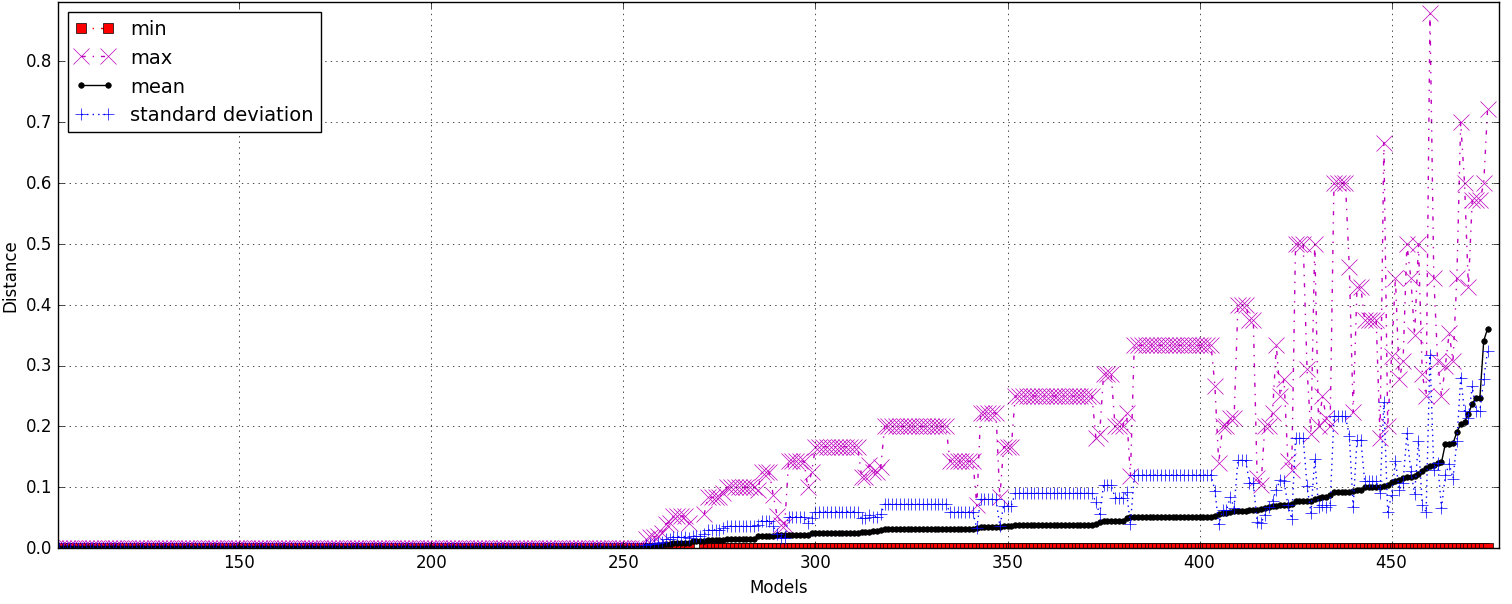
\includegraphics[width=\textwidth]{figs/jacdis2.png} \\
  \caption{Pairwise Jaccard distance between IVCs}\label{fig:jacdis}
\end{figure*}

\subsection{Diversity}
\label{sec:diversity}
Recall from Section~\ref{sec:ivc} that a {\em minimal} core is any core leading to a proof such that if you remove any of the conjuncts from the core, it no longer produces a proof.  For certain models and properties, it is possible that there are many minimal cores that will lead to a proof.  In this section, we examine the issue of diversity: do different tools and algorithms lead to {\em different} minimal cores?  This is both a function of the models and the solution algorithms: for certain models, there is only one possible minimal core, whereas other models might have many. Given that there are multiple solutions, the interesting question is whether using different tools and algorithms will lead to different solutions.  Note that this question is closely tied to that of {\em minimality}, which we examined in the previous section.

Our exploration in this case is not exhaustive, but only exploratory.  The reason it is considered is that it has substantial relevance to some of the uses of the tool: e.g., for constructing traceability matrices from proofs.  Given diversity of results, we may wish to distinguish {\em must} traceability elements from {\em may} traceability elements across a set of diverse solutions, and consider more systematic explorations of diversity in future work.

To measure diversity of IVCs, we use Jaccard distance:
\begin{definition}{\emph{Jaccard distance:}}
  \label{def:dj}
  $d_J(\small{A}, \small{B}) = 1 - \frac{|A \cap B|}{|A \cup B|} ,\\ 0 \leq d_J(\small{A}, \small{B}) \leq 1$
\end{definition}
\noindent Jaccard distance is a standard metric for comparing finite sets (assuming that both sets are non-empty) by comparing the size of the intersection of two sets over its union.  For each model in the benchmark, the experiments generated 13 different sets of support. Therefore, we obtained $\binom{13}{2} = 78$ combinations of pairwise distances per model. Then, minimum, maximum, average, and standard deviation of the distances were calculated (Fig~\ref{fig:jacdis}), by which, again, we calculated these four measures among all models.  As seen in Table~\ref{tab:jaccard-avg}, on average, the Jaccard distance between different solutions is small, but the maximum is close to 1, which indicates that even for our exploratory analysis, there are models for which the tools yield substantially diverse solutions.  The diversity between solutions is represented graphically in Figure~\ref{fig:jacdis}, where for each model, we present the min, max, and mean pairwise distance of the solutions produced by algorithm \ucalg for each model, ranked by the mean distance.

\iffalse
\mike{Do we want the discussion below?  I am not sure that it adds much}

To measure the overall similarity among all sets, instead of a pairwise comparison, we used \emph{frequent pattern mining} \cite{han2007frequent}. To define an overall similarity among all sets of support of a given model\footnote{Note that all models in the benchmarks are single property; hence, instead of saying a set of support of a given \emph{property}, we just refer it as the support set of the \emph{model} while explaining the experimental results.}, we calculated a \emph{core} support set for each model in the benchmark, which can be considered as a closed frequent pattern; a core set of model $M$, denoted by $C_M$, is defined as:
\begin{definition}
  \label{def:core}
  $C_M = \bigcap_{i=1}^{13} s_{Mi},   \hspace{9pt} s_{Mi} \in S_M$
\end{definition}

Based on this notion, overall dissimilarity, denoted by $D_{J\{M\}}$, is defined as follows:

\begin{definition}
  \label{def:dis}
  $D_{J\{M\}} =  \frac{\sum_{i=1}^{12}d_J(s_{Mi}, C_M)}{12},   \hspace{9pt} s_{Mi} \in S_M$
\end{definition}

Since our goal is to measure the diversity or dissimilarity among sets computed by \texttt{ReduceSupport}, in \ref{def:dis}, we exclude the set generated by \texttt{JSupport}. In Fig~\ref{fig:jacdis}, the \emph{overall distance} line shows $D_{J\{M\}}$ per model, which can be analyzed from the following hypotheses:
\begin{itemize}
  \item H0: variety of obtained sets of support is high (average $D_{J\{M\}}$ of 0.2)
  \item H1: variety of obtained sets of support is small (average $D_{J\{M\}}$ less than 0.2)
\end{itemize}
Table~\ref{tab:variety} shows that, with an effect size of 0.79, H0 can be rejected.
\begin{table}
  \centering
  \begin{tabular}{ |c|c|c|c|c|c| }
    \hline
     min & max & mean & stdev & ES & p-value\\[0.5ex]
    \hline
    %sample size = 395
     0.0   & 0.879 & 0.099 & 0.141 & 0.72 & < 0.00001 \\[0.5ex]
    \hline
  \end{tabular}
  \caption{$D_{J\{M\}}$ among all models}
  \label{tab:variety}
\end{table}
\fi
%summarized as follows:
%\begin{itemize}
%  \item minimum $D_{J\{M\}}$ among all models: 0.0
%  \item maximum $D_{J\{M\}}$ among all models: 0.879
%  \item average $D_{J\{M\}}$ among all models: 0.096
%  \item standard deviation of $D_{J\{M\}}$ among all models: 0.132
%\end{itemize}


\subsection{Discussion}

In the previous section, we presented three algorithms for determining inductive validity cores.  The brute-force algorithm is guaranteed minimal, but is often very slow.  The other two algorithms: the UNSAT-core algorithm \ucalg\ and the combined algorithm \ucbfalg, represent interesting trade-offs.  The \ucalg\ algorithm is much faster, but is not guaranteed to be minimal; the result of this algorithm can be further, and often quite quickly, refined by the combined algorithm.  Thus, we can choose to trade off speed for guaranteed minimality using these two algorithms; the combined algorithm can be viewed as a refinement algorithm that we can terminate either at completion or after a fixed time bound.


%One question that arises is: why is the refinement so much quicker than the brute-force approach?  In our preliminary examination, it appears to be because of the actions performed by JKind on the sub-problems.  When the cores produced by \ucalg\ are minimal or close to minimal, it tends to be the case that removing conjuncts from the core leads to short counterexamples.  When performing the brute-force algorithm, removing the irrelevant pieces of the model require repeated proof search.

Although our experiment does not ask statistical questions, it is still worth examining threats towards generalizing our results.  First, are the models and properties that we chose representative?  We started from an existing benchmark from another research group suite to try to assuage this concern, but most of these models were small, so we extended the benchmark suite with 81 of our own models.  It is possible that our additions skew the results, though these models are immediately derived from previously published work and not modified for our analysis here.  Second, our models and tools use the Lustre language, which is equational, rather than conjuncted transition systems; it is possible (though, in our opinion, unlikely) that arbitrary conjuncts rather than equations will yield different performance or minimality characteristics.



\section{Experiments on the Online method of computing AIVCs}
We are interested in examining the performance of algorithms to compute minimal IVCs.
We examine \textbf{Grow-Shrink}, the algorithm presented in Section \ref{sec:onaivc}, and the two state-of-the-art algorithms: \textbf{Offline MARCO} (\aivcalg Section \ref{sec:offaivc}), and \textbf{Online MARCO} (Section \ref{sec:onaivc}) that performs a shrink step prior to returning a solution to ensure minimality.
%\old{We examine three algorithms:
%\textbf{Offline MARCO}, the algorithm from~\cite{Ghass17AllIVCs}, \textbf{Online MARCO}, a variant of the algorithm from~\cite{Ghass17AllIVCs} that performs a shrink step prior to returning a solution to ensure minimality, and \textbf{Grow-Shrink}, the algorithm described in this paper.}
We investigate the following research questions: 
\begin{itemize}
  \item \textbf{RQ1:} For the large models where the complete MIVC enumeration is intractable,
how many MIVCs are found within the given time limit? 
  \item \textbf{RQ2:} For the tractable models, i.e. models in which all MIVCs are found, how much time is required to complete the enumeration of MIVCs?
  \item \textbf{RQ3:} Finally, we are interested in how many solver calls are necessary for the enumeration. What is the (average) number of solver calls with result adequate/inadequate required by evaluated online algorithms to produce individual MIVCs?
\end{itemize}

\subsection{Experimental Setup}
  We start from a benchmark suite that is a superset of the benchmarks used in the previous experiments. This suite contains 660 models, and includes all models that yield a valid result (530 in total) from previous Lustre model checking papers~\cite{Hagen08:FMCAD,piskac2016} and 130 industrial models yielding valid results derived from an infusion pump system \cite{hilt2013} and other sources \cite{piskac2016,NFM2015:backes}.
As this paper is concerned with analysis problems involving multiple MIVCs, we include only models that had more than 4 MIVCs (46 models in total).  To consider problems with many IVCs, we took those models and mutated them, constructing 20 mutants for each model. The mutants varied both in the number and in the size of individual MIVCs.
We added the mutants that still yielded valid results and have more than 5 MIVCs (384 in total) back to the benchmark suite.
Thus, the final suite contains 430 Lustre models. The original benchmarks and our augmented benchmark are available online\footnote{\url{https://github.com/elaghs/benchmarks}}.
%\cite{bench}.

For each test model, we configured \texttt{JKind} to use the \texttt{Z3} solver and the ``fastest'' mode of \texttt{JKind} (which involves running the $k$-induction and PDR engines in parallel and terminating when a solution is found). The experiments were run on a  3.50GHz  Intel(R) i5-4690 processor 16 GB memory machine running Linux with a 30 minute timeout.  All experimental data is available online\footnote{\url{https://github.com/jar-ben/online-mivc-enumeration}}.
%~\cite{expr}.




\begin{figure}
\centering
\begin{minipage}{\textwidth}
\centering
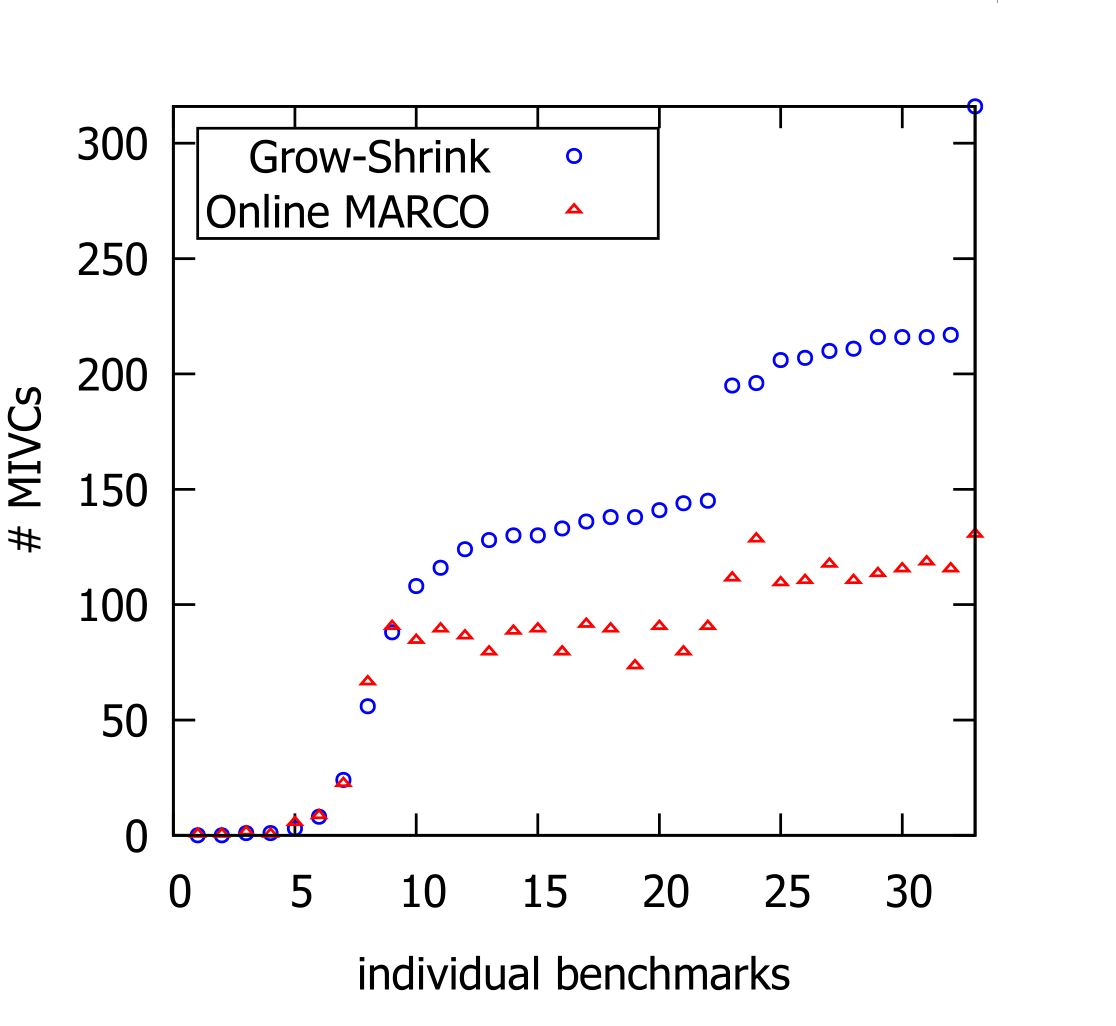
\includegraphics[scale=0.5]{./figs/found_mivcs.png}%
\captionof{figure}{Number of MIVCs produced by online algorithms.}%
\label{res:found_mivcs}
\end{minipage}\hfill
\begin{minipage}{\textwidth}
\centering
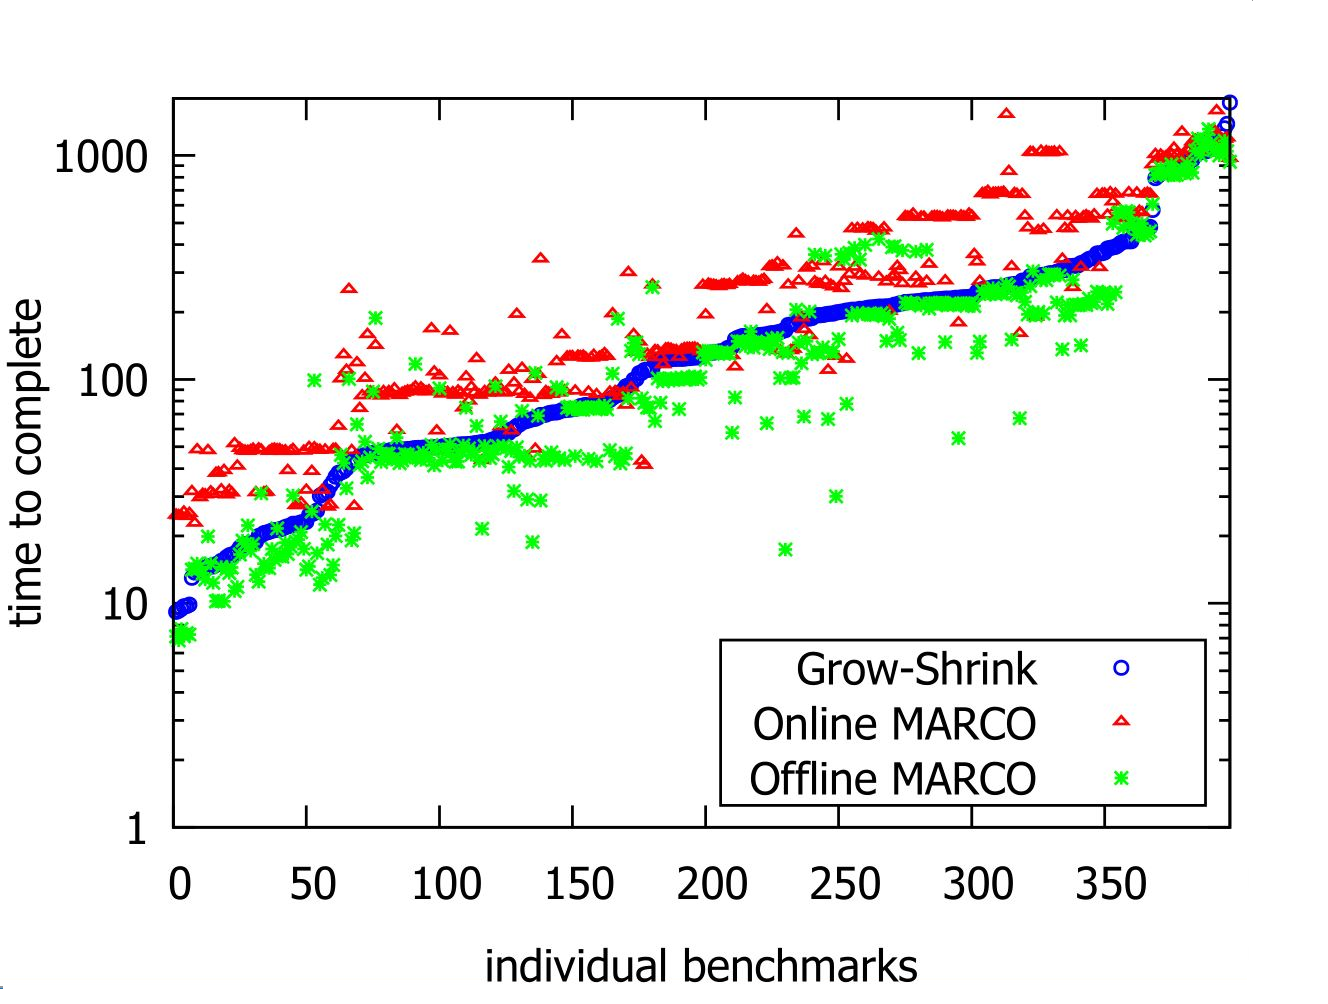
\includegraphics[scale=0.5]{./figs/time_to_complete.png}%
\captionof{figure}{Runtime for tractable benchmarks for all algorithms in a log scale.}%
\label{res:time_to_complete}
\end{minipage}
\end{figure}



\subsection{Experimental Results}
In this section, we examine the experimental results to address the research questions.

%\vspace{-5pt}
vspace{0.1in}
\subsubsection{RQ1 and RQ2}
Data related to the first two research questions are shown in Figures~\ref{res:found_mivcs} and~\ref{res:time_to_complete}.
Figure~\ref{res:found_mivcs} describes the number of MIVCs found be the two online algorithms in the intractable benchmarks, i.e. the benchmarks where the algorithms did not complete the computation within the time limit. There are 33 such benchmarks. The Grow-Shrink substantially outperforms Online MARCO in the majority of the benchmarks, finding an average of 55\% additional MIVCs.

Figure~\ref{res:time_to_complete} describes the time for each algorithm needed to complete the computation in the case of 397 tractable benchmarks.

Grow-Shrink is on
average only 1.08 times slower than Offline MARCO,
yet as previously discussed,
has the advantage of returning guaranteed MIVCs,
rather than approximate MIVCs.
It is on average 1.50 times faster than Online MARCO.


%It is much faster than the Online MARCO algorithm.


%\vspace{-5pt}
vspace{0.1in}
\subsubsection{RQ3}  For RQ3, we examined the number of required calls to the solver per MIVC.  For this question, we used the 33 models that contained a large number of MIVCs ($>$70) in order to show the solver efficiency as the number of MIVCs increased.  A point with coordinates $(x,y)$ states that the algorithm needed to perform $y$ solver calls (on average) in order to produce (find) the first $x$ MIVCs. We grouped the calls in terms of the number of calls that returned {\em adequate} vs. {\em inadequate} results.  It is evidenced by the results in Figure~\ref{res:checks}, the new algorithm improves upon Online MARCO as the number of MIVCs becomes larger.

\begin{figure}
\centering
\begin{subfigure}{\textwidth}
  \centering
  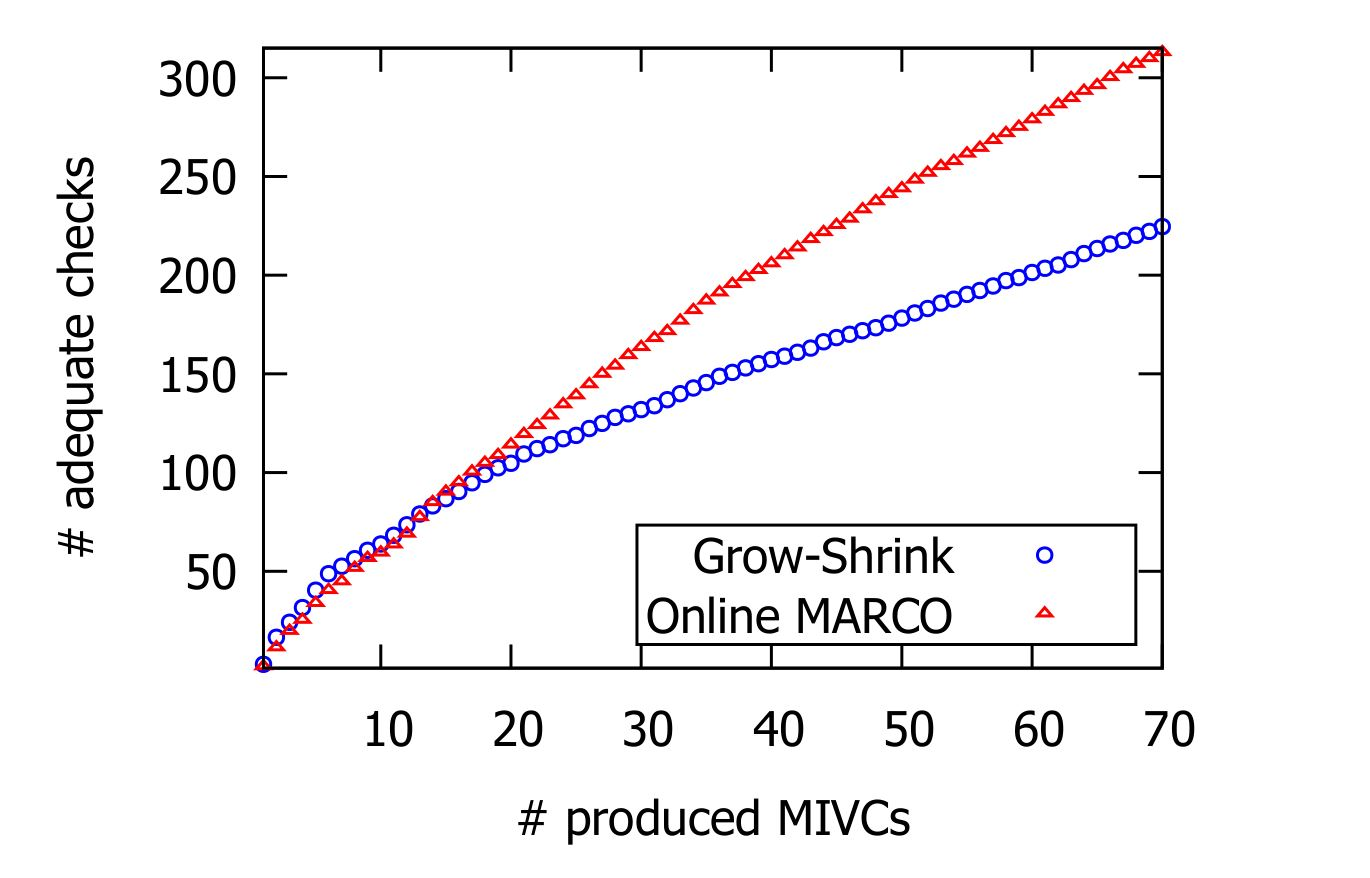
\includegraphics[scale=0.5]{./figs/adequate_checks_per_mivc_70.png}
  \caption{Checks with result "adequate".}
  \label{res:adequate_checks} 
\end{subfigure}\hfill
\begin{subfigure}{\textwidth}
  \centering
  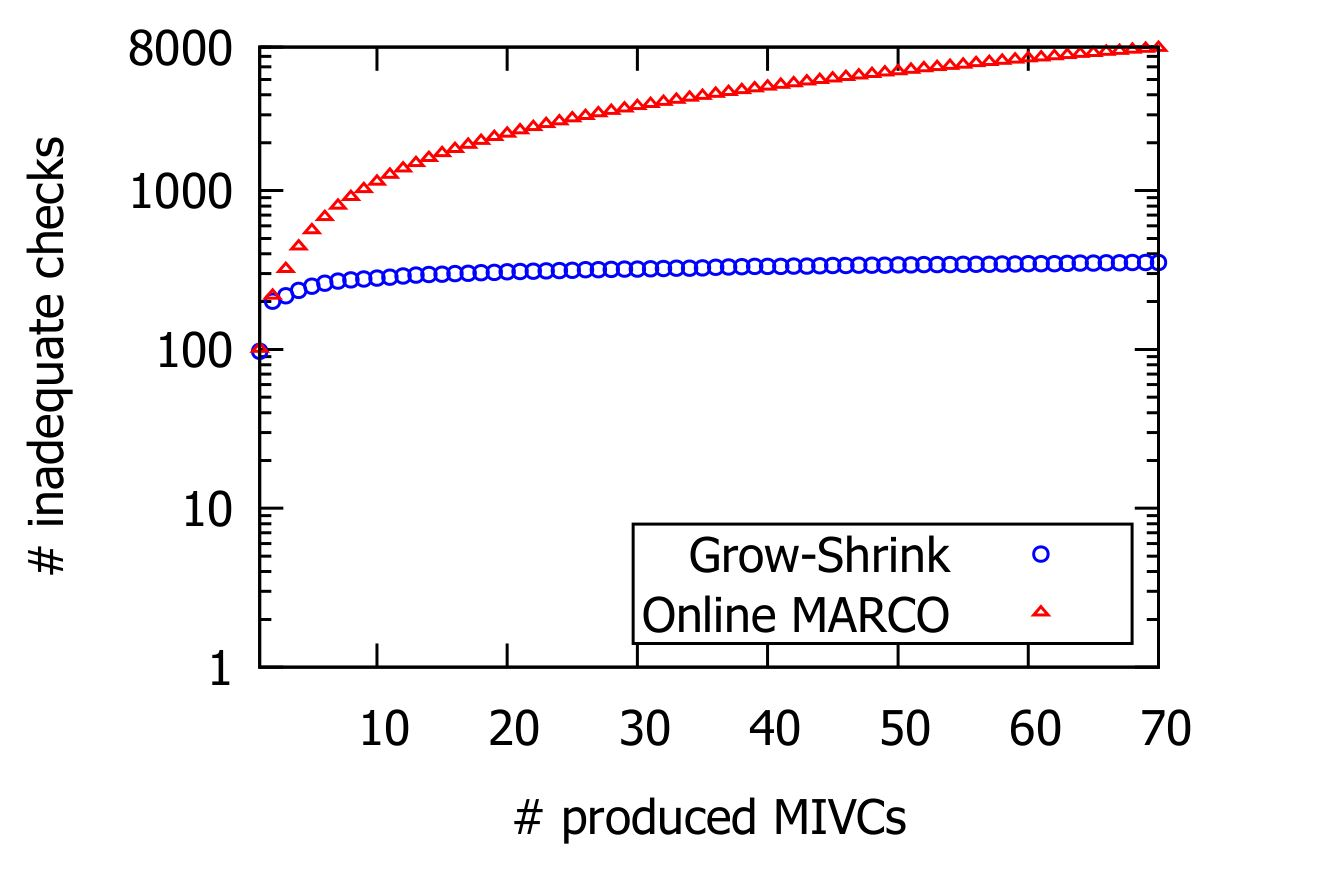
\includegraphics[scale=0.5]{./figs/inadequate_checks_per_mivc_70.png}
  \caption{Checks with result "inadequate".}
  \label{res:inadequate_checks}
\end{subfigure}
\caption{Average number of performed adequacy checks required to produce individual MIVCs. Note that Figure (b) is in a log scale.}
\label{res:checks}
\end{figure}

The improvement in the number of \emph{inadequate} calls is due the novel shrinking and growing procedures.
Each (approximately) maximal inadequate subset found by the growing procedure allows to save (up to exponentially) many inadequate calls during subsequent executions of the shrinking procedure.
Indeed, the Grow-Shrink algorithm performed on average only 353 inadequate calls to output the first 70 MIVCs, whereas the online MARCO needed to perform 7775 calls to output the same number of MIVCs.

The improvement in the number of \emph{adequate} calls is not so significant as in the case of inadequate calls. Yet, since the adequate calls are usually much more time consuming than inadequate ones, even a slight saving in the number of adequate calls might significantly speed up the whole computation. The Grow-Shrink algorithm saves adequate calls due to the usage of the shrinking queue and due to the invariants that are maintained by the queue. In particular, shall two comparable sets appear in the queue, only the smaller is left. Thus, the algorithm avoids shrinking of relatively large sets and saves some adequate calls.



\section{Experiments on BVCs}
We would like to to observe and study how validity cores evolves over unrolling the transition relation. It is interesting to see how quickly validity cores from a bounded proof converges to an actual minimal IVC.

Note that the purpose of our experiments on BVCs is mostly to point out some research directions. Further studies may even can make use of BVCs in verification problems. It can be the case that a valid property is hard or impossible for an inductive model checker to prove. In such cases, looking at the history of BVC runs may give us some confidence about the correctness of the property. The experimental results show that when we reach one of the actual MIVCs, the BVC algorithm then constantly generates the same cores as depth of exploration increases. That is to say, when the BVC runs begin generating stable cores that do not change as depth changes, it may imply we might have already seen all the reachable states, and implicitly known they are safe. Although this hypothesis is by no means guaranteed to hold, it may be worth further investigations.

\subsection{Experimental Setup}
  We perform our experiments on the same benchmark suite with 660 models introduced in Section \ref{sec:expsetup}. The experiment is conducted with a maximum depth of 10 and one hour timeout; i.e., for each model, if unrolling to depth 10 takes more than one hour, the \bvcalg\ algorithm will terminate. We capture $\bvc _{k}$ for $ 0 \leq k \le 10$, then compare each \bvc\ of depth $k$ to see how they change during unrolling. Then, the final bounded validity cores obtained from at the maximum\footnote{Maximum depth in this experiment is 10. For most of the models, it is possible to reach this depth in less than an hour.}
  reachable depth in one hour, denoted by $\bvc _{max}$ , are considered as our final cores. These cores are compared with all the MIVCs gathered in Section \ref{subsec:res} to see if they match up with any of the actual minimal IVCs.

Research questions we would like to answer in this study are as follows:
\begin{itemize}
  \item \textbf{RQ1:} How many of the final \bvc s match one of the \mivc s?
  %How many of the final BVCs do match up with one of the MIVCs? For how many of the models does the algorithm time out?
  \item \textbf{RQ2:} How do \bvc s evolve as the analysis depth changes?
  %At what rate does size of the BVCs change? Does the size of the cores increase with the depth?
  \item \textbf{RQ3:} Is there a relationship between size and structure of models and the size of \bvc s and the rate at which they converge with a \mivc?
  %How close is $\bvc _{max}$ to an actual MIVC? Is there any relationship with the size of the models and convergence of the BVCs?
\end{itemize}

\vspace{0.1in}
\subsubsection{RQ1}
The result of the experiments show that $\bvc _{max}$ is the same as one of the MIVCs for 474 models out of 660. For 27 of the models, $\bvc _{max}$ was not subset of any MIVCs (had additional elements, also none of the MIVCs was a subset of the $\bvc _{max}$)\footnote{We will explain the reason in \textbf{RQ2}}. However, $\bvc _{max}$ was a subset of one of the MIVCs in 159 of the models.

We performed the experiments with \texttt{Z3} and \texttt{Yices} solvers. UNSAT core generation in \texttt{Z3} is faster than \texttt{Yices} in the current implementation of \texttt{JKind}. Using \texttt{Z3}, 12 of the models did not reach depth 10 in one hour. With \texttt{Yices}, 18 of the models timed out. An interesting fact is that we had models that did not reach $\bvc _{10}$, but their $\bvc _{max}$ was the same as one of the MIVCs. For example, one of the models containing 571 design elements only reached to $\bvc _{2}$, but $\bvc _{2}$ was the same as one of the MIVCs.
The BVC size for that model at different depths is as follows:\footnote{This particular model is named ``steam\_boiler\_no\_arr1.lus'' in our benchmarks. You can see the results and model in our experimental directories \cite{expr}.}

$|\bvc _{0}| = 6$, $|\bvc _{1}| = 11$, $|\bvc _{2}| = 128$

There are interesting case studies where from the initial depth, the BVC was the same as one of the MIVCs. For example, in our benchmark we have a model with 27 design elements\footnote{File ``car\_all\_e8\_856\_e2\_585.lus'' in our benchmark directory.}, for which $|\bvc _{i}| = 5$, $i \leq 0 \le 10$, and $\bvc _{0}$ is the same as its only one MIVC.

\vspace{0.1in}
\subsubsection{RQ2}
Our experimental results show that among 474 models for which $\bvc _{max}$ is the same as one of the MIVCs, the size of the BVCs were (nonstrictly) increasing 99.9\% of the time:
      $$ 0 \leq i \le max, |\bvc _{i}| \leq |\bvc _{i+1}|$$
      In other words, for only 12 of these models, the above relation did not hold.
      It is expected that bounded cores in each unrolling step (nonstrictly) increase as in each step more states are being reached and the cores required for the proof of the property is more likely to expand.
      We run the experiments over those 12 models with different solvers (once with \texttt{Z3} and once with \texttt{Yices}). The result of BVC runs for these models (on \texttt{Yices}) is shown in Table \ref{tab:bvc-abnormal}.

      It is interesting to see why those 12 models show different behavior. By looking at different case studies, we have found three main reasons that explain this anomaly.  The first explanation is that when a model has several distinct MIVCs, the bounded core could change during unrolling. However, the set of 12 models contain models that have only a single MIVC, so this cannot be the entire reason. Another explanation for such models is that MIVCs obtained from \aivcalg ~contained timeout loops; therefore, we do not have the exact minimal IVCs for those cases (for example model\#6 in Table \ref{tab:bvc-abnormal}).




      % (a) shows a picture containing all the models. Figure  \ref{fig:bvc-growth} (b) is the enlarged version for some of the smaller models, and Figure  \ref{fig:bvc-growth} (c) magnifies the parts for larger models.



\begin{table}
  \caption{BVC runs for the models with non-increasing behavior where $\bvc _{max}$ is the same as one of the MIVCs.}

  \centering
  \begin{tabularx}{\linewidth}{ |c||c|c|c|c|c|c|c|c|c|c||L|L|}
    \hline
    $|\bvc _{i}|$ ~/~ $i=$ & 0 & 1 & 2 & 3 & 4 & 5 & 6 & 7 & 8 & 9 & \small{model size} & \small{\#of MIVCs} \\[0.5ex]
    \hline\hline

    model\#1& 2 & 9 & 34 & 36& 28 & 28 & 28 & 28 & 28 & 28 & 70&1 \\[0.5ex]
    model\#2& 5 & 15 & 11& 11& 11 & 11 & 11 & 11 & 11 & 11 & 123 &1\\[0.5ex]
    model\#3& 8 & 9& 13& 33& 28& 40& 38& 41& 41& 41&57 &7 \\[0.5ex]
    model\#4& 2& 5& 8& 10& 12& 10& 10& 10& 10& 10 &64 &9\\[0.5ex]
    \small{model\#5 (\texttt{Yices})}&9& 24 & 84& 84& 82& 82& 82& 82& 82& 82&96 &1\\[0.5ex]
    \small{model\#5 (\texttt{Z3})}& 9& 24& 82& 82& 82& 82& 82& 82& 82& 82&96 &1\\[0.5ex]
    model\#6& 5& 6& 5& 7& 5& 7& 5& 7& 5& 7& 7 &1\\[0.5ex]
    model\#7& 5& 6& 6& 5& 5& 6& 6& 5& 5& 6&6 &1\\[0.5ex]
    \small{model\#8 (\texttt{Yices})}& 9& 12& 14& 28& 37& 36& 36& 36& 36& 36&103&1 \\[0.5ex]
    \small{model\#8 (\texttt{Z3})}&9& 12& 14& 28& 37& 37& 37& 37& 37& 37& 103&1\\[0.5ex]
    \small{model\#9 (\texttt{Yices})}& 2& 6& 10& 4& 4& 4& 4& 4& 4& 4 &64&1 \\[0.5ex]
    \small{model\#9 (\texttt{Z3})}& 2& 4& 4& 4& 4& 4& 4& 4& 4& 4 &64&1\\[0.5ex]
    model\#10& 2& 6& 8& 11& 7& 7& 7& 7& 7& 7 &64&1\\[0.5ex]
    model\#11& 4& 13& 32& 47& 61& 54& 54& 54& 54& 54 &103&8 \\[0.5ex]
 \small{model\#12 (\texttt{Yices})}& 8& 8& 21& 29& 39& 38& 38& 40& 41& 41&57&6\\[0.5ex]
  \small{model\#12 (\texttt{Z3})}& 8& 17& 21& 29& 32& 38& 38& 32& 32& 32&57&6 \\[0.5ex]
    \hline
  \end{tabularx} \\
%{Actual model names in Table \ref{tab:bvc-abnormal}\\model\#1: fast\_1\_e8\_751.lus \\model\#2: microwave05.lus\\mode\#3: DRAGON\_12.lus\\model\#4: Display\_Control-Gaurantee0
%  \\model\#5:fast\_2\_e8\_976.lus
%  \\model\#6: twisted\_counters.lus
%  \\model\#7: two\_counters.lus
%  \\model\#8: cruise\_controller\_04.lus
%  \\model\#9: Display\_Control-Gaurantee2.lus
%  \\model\#10: Display\_Control-Gaurantee1.lus
%  \\model\#11: cruise\_controller\_24.lus
%  \\model\#12: DRAGON\_13.lus}
\vspace{0.07in}
{\small{Actual model names in the benchmark, respectively: fast\_1\_e8\_751.lus, microwave05.lus, DRAGON\_12.lus, Display\_Control-Gaurantee0, fast\_2\_e8\_976.lus, twisted\_counters.lus, two\_counters.lus, cruise\_controller\_04.lus, Display\_Control-Gaurantee2.lus, Display\_Control-Gaurantee1.lus, cruise\_controller\_24.lus, DRAGON\_13.lus}}
  \label{tab:bvc-abnormal}
\end{table}

The third reason why the size of BVCs is not always increasing is more interesting.   This reason explains why in some cases $\bvc _{max}$ is not the subset of any of the MIVCs. This only has to do with the depth of bounded model checking. In some problems, when we are at the earlier steps of unrolling transition relation (i.e., lower depths), the property can be satisfied in different ways. In other words, a property may have multiple \bvc s at depth $k$, but as we advance towards the deeper bounds leading to a proof, the validity cores converge to a smaller subset. For example, consider the toy example in Figure \ref{fig:toybvc}. It shows a simple model containing two counters. The first counter ({\small{\texttt{counter1}}}) has the initial value of 0, and the second counter ({\small{\texttt{counter2}}}) starts off from 6. The property ({\small{\texttt{OK}}}) is either {\small{\texttt{counter1}}} is less than 5 or ({\small{\texttt{counter2}}}) is greater than 5. This property has only one MIVC, which is {\small{\texttt{\{counter2, OK\}}}}. However, before depth 5, this property can be satisfied into ways with {\small{\texttt{\{counter1, OK\}}}} and {\small{\texttt{\{counter2, OK\}}}}. You can see the output of the BVC engine for this example in Figure \ref{fig:toyo1}.

\begin{figure}
 \centering
  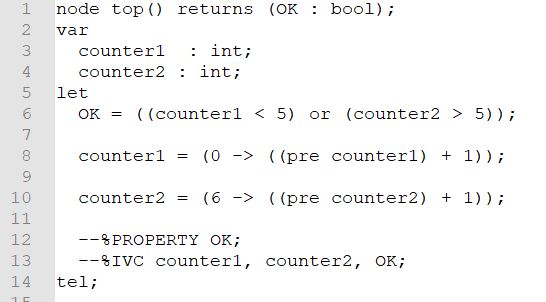
\includegraphics[width=0.8\columnwidth]{figs/toybvc.jpg}
  %\vspace{-0.1in}
  \caption{A toy example that shows multiple BVCs at earlier depths for a property with single MIVC}
  \vspace{0.1in}
  \label{fig:toybvc}
\end{figure}

\begin{figure}
 \centering
  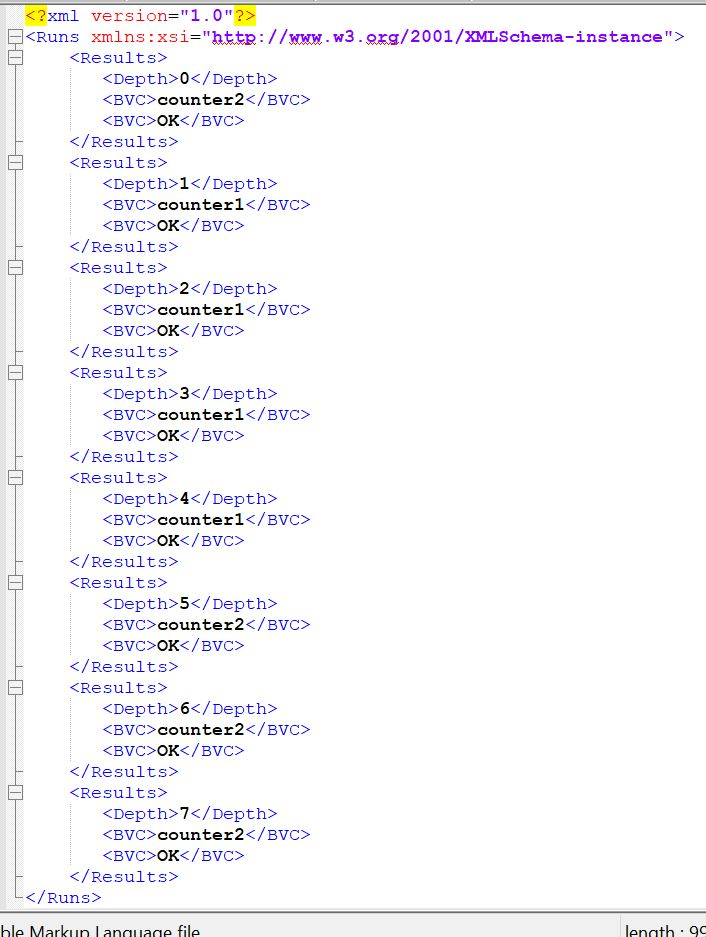
\includegraphics[width=0.8\columnwidth]{figs/toyo1.jpg}
  %\vspace{-0.1in}
  \caption{BVCs for the property in Figure \ref{fig:toybvc}}
  \vspace{0.1in}
  \label{fig:toyo1}
\end{figure}



Let us take a look at one of the models that is small enough to display its results in a reasonable amount of space. This model is named \emph{ex3\_e8\_381\_e7\_224} in our benchmarks (Figure \ref{fig:expl}). It only has one MIVC ({\small{\texttt{\{V19\_late, V64\_incr, V63\_diff, V65\_PC, OK\}}}}), and \jkind is able to prove its property in less than a second. In addition, for this model, there is no timeout issue in the inner loops of \aivcalg\ algorithm. Using \texttt{Yices} in our experiments, $\bvc _{max}$ is not the subset of the only MIVC that this model has. However if we had just increased the depth by 1, from $\bvc _{10}$ on, the BVC would have become the same as the MIVC. For this model, up to depth 10, we have two ways of satisfying the property (we have two bounded validity cores {\small{\texttt{\{V19\_late, V64\_incr, V63\_diff, V65\_PC, OK\}}}} and {\small{\texttt{\{V20\_early, V64\_incr, V63\_diff, V65\_PC, OK\}}}}), but after depth 10, the property is satisfied with only one validity core ({\small{\texttt{\{V19\_late, V64\_incr, V63\_diff, V65\_PC, OK\}}}}). Figure \ref{fig:explout} shows the output of the \jkind BVC engine over this model up to depth 15.

 \begin{figure}
 \centering
  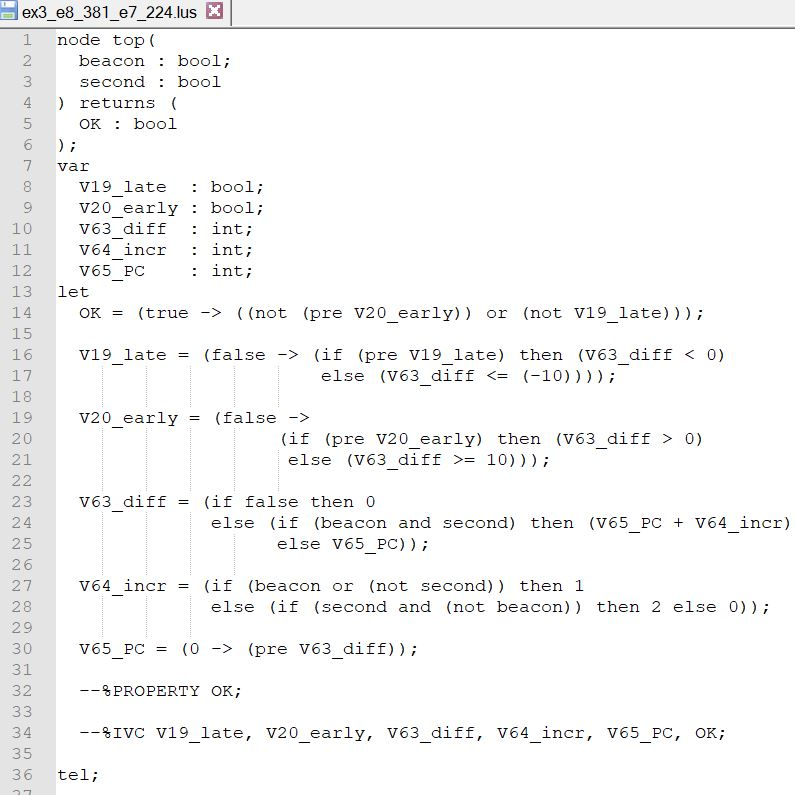
\includegraphics[width=0.9\columnwidth]{figs/expl.jpg}
  %\vspace{-0.1in}
  \caption{Model ex3\_e8\_381\_e7\_224 as a case study}
  \vspace{0.1in}
  \label{fig:expl}
\end{figure}

\begin{figure}
 \centering
  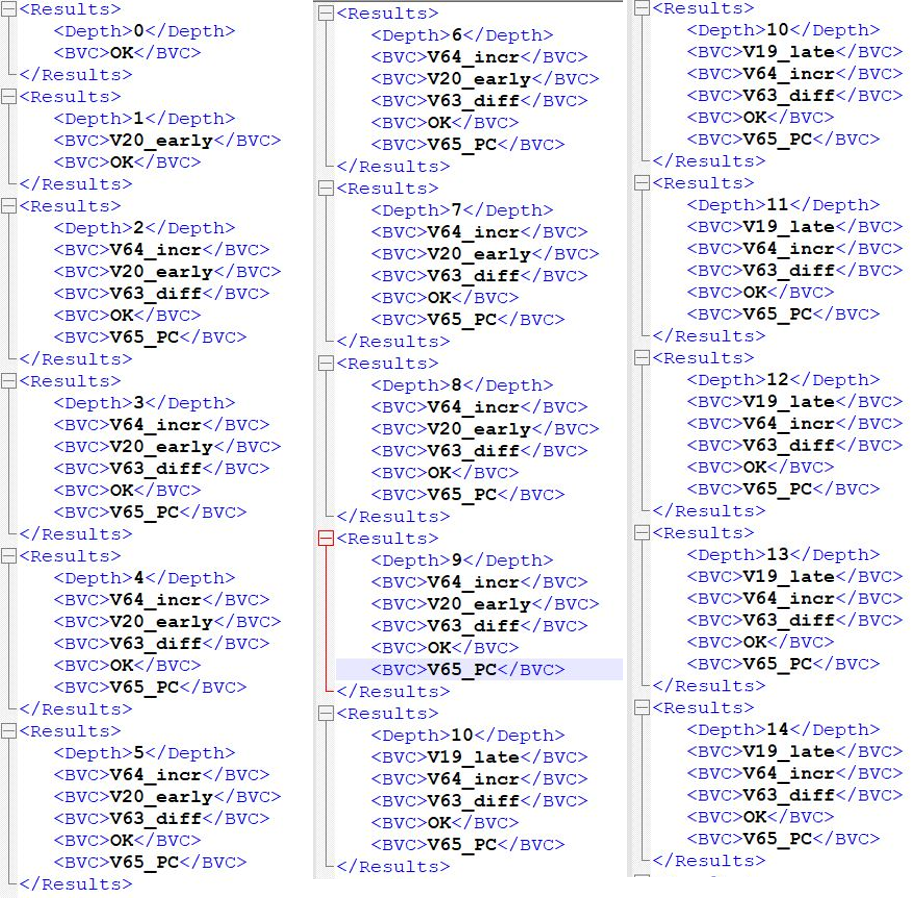
\includegraphics[width=0.9\columnwidth]{figs/explout.png}
  %\vspace{-0.1in}
  \caption{BVC runs for model ex3\_e8\_381\_e7\_224}
  \vspace{0.1in}
  \label{fig:explout}
\end{figure}


\vspace{0.1in}
\subsubsection{RQ3}
In order to show how quickly BVCs change and converge to an actual MIVC, we chose $\bvc _{0}$, $\bvc _{3}$, and $\bvc _{max}$  runs and plot the size of the cores. Mostly for models with less than 200 design elements, size of BVCs did not change much from depth 3 to 9. For the larger models there is some difference between the size of $\bvc _{3}$ and $\bvc _{max}$ (Figure \ref{fig:bvc-growth}).


 \begin{figure}
 \centering
  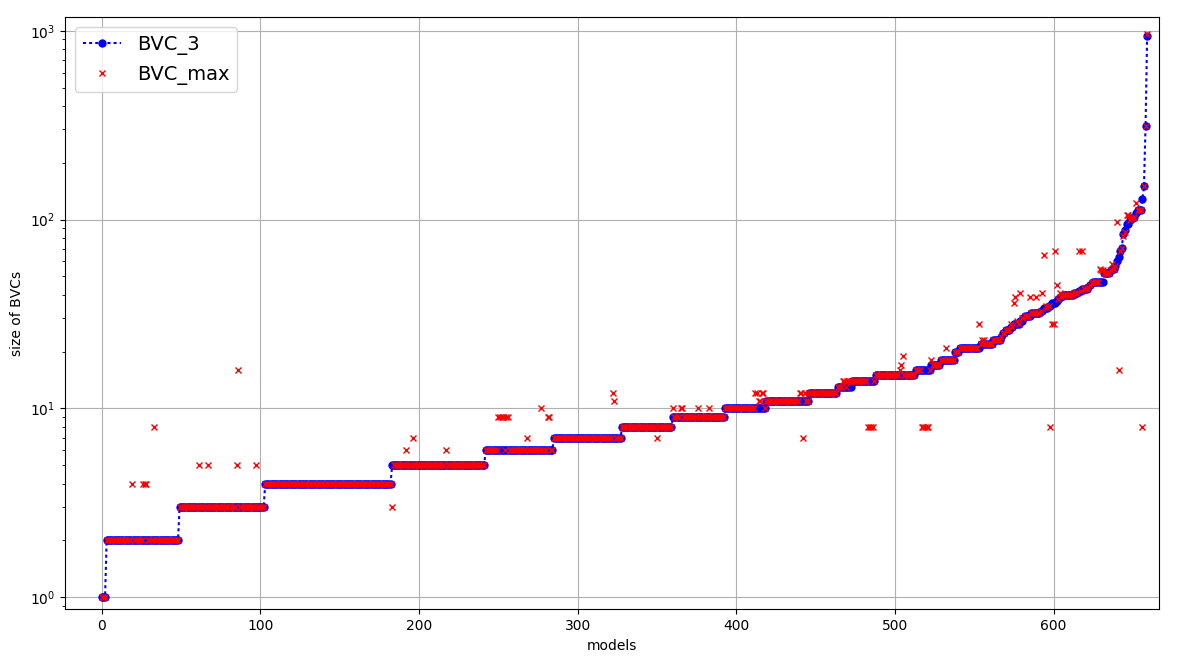
\includegraphics[width=.85\columnwidth]{figs/bvcmax.png}
  %\vspace{-0.1in}
  \caption{Size of BVCs at depth 3 and max}
  \vspace{0.1in}
  \label{fig:bvc-growth}
\end{figure}


We calculated the difference of $\bvc _{max}$ of each model with its MIVCs. Part of the results is described in \textbf{RQ1}. If $\bvc _{max}$  is the subset of one of the MIVCs, we calculated the difference between those two, and if not, $\bvc _{max}$  is compared with one of the MIVCs of the model, selected randomly.  Note that it is possible for $\bvc _{max}$ to be a subset of more than one of the MIVCs. In our calculation, we randomly selected the first MIVC containing $\bvc _{max}$.
%Figure \ref{fig:dif-bvc} visualizes the results.
Figure \ref{fig:bvc-size} shows the size of the models versus the size differences of MIVCs and BVCs
%line from Figure \ref{fig:dif-bvc}
in logarithmic scale.

% \begin{figure}
% \centering
%  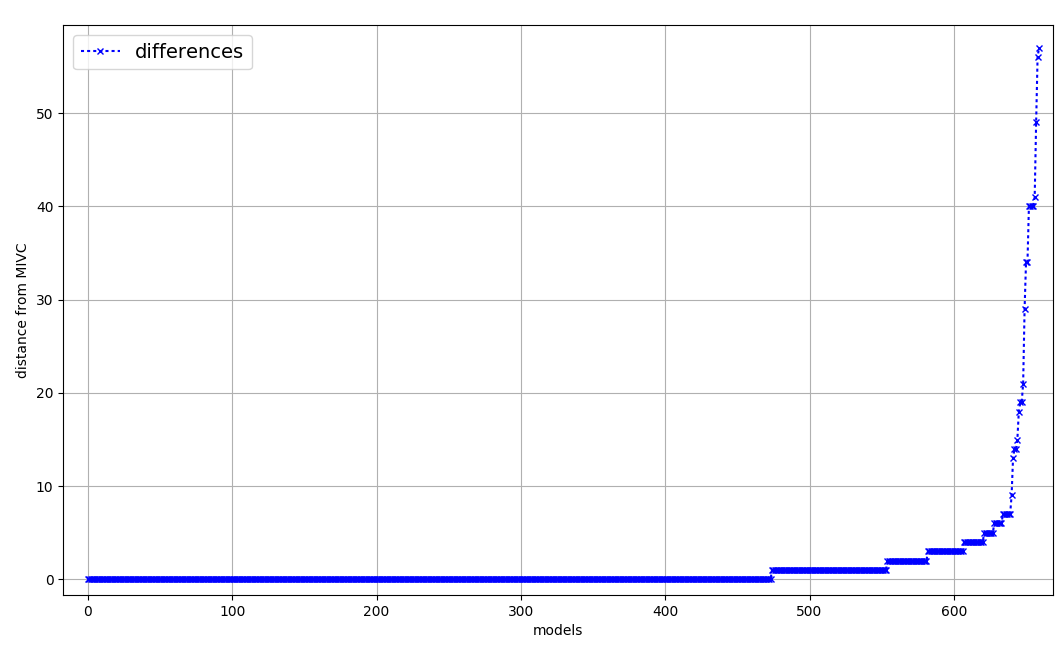
\includegraphics[width=\columnwidth]{figs/bvc_dif_yices.png}
%  %\vspace{-0.1in}
%  \caption{Difference between $\bvc _{max}$ and MIVCs}
%  \vspace{0.1in}
%  \label{fig:dif-bvc}
%\end{figure}

 \begin{figure}
 \centering
  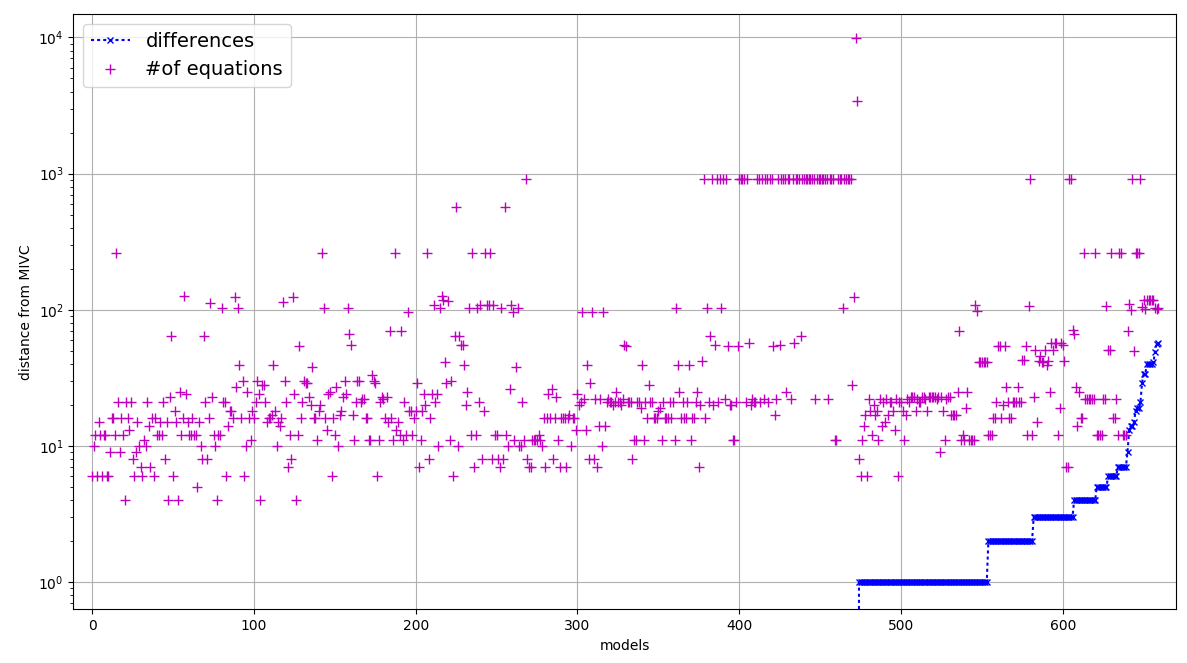
\includegraphics[width=\columnwidth]{figs/bvc_modelsize_yices.png}
  %\vspace{-0.1in}
  \caption{Difference between $\bvc _{max}$ and MIVCs vs the model size}
  \vspace{0.1in}
  \label{fig:bvc-size}
\end{figure}

\vspace{0.1in}
\subsubsection{Discussion}
Experimental results show that in many cases, bounded validity cores can be as accurate as actual minimal IVCs. The abnormal behavior in some cases showed that we cannot make a strong claim about the relationships between BVCs and IVCs. One observation is that at deeper bounds, we can have more accurate bounded validity cores. The more accurate bounded cores are, the more useful information we have to evaluate completeness and adequacy of proofs.

It may be possible to make use of other techniques to evaluate the accuracy of the bounded cores. For example, in case of non-increasing BVCs, we may build different abstractions for the model using different BVCs, and try to prove the property over abstracted models. If property fails over one abstraction, we can easily rule out the bounded core used for that abstraction. For example, in Figure \ref{fig:toybvc}, if we terminate the BVC generation at depth 4, we need to decide which of {\small{\texttt{\{counter1, OK\}}}} and {\small{\texttt{\{counter2, OK\}}}} is necessary for an inductive proof (i.e., is the subset of our MIVC). In order to do so, if we build a new abstract model using BVC {\small{\texttt{\{counter1, OK\}}}} (Figure \ref{fig:absbvc} (a)), and try to re-prove the property, property will be violated, which tells us   {\small{\texttt{counter2}}} was necessary for the proof of our property. In the same way, if we build an abstract model using BVC  {\small{\texttt{\{counter2, OK\}}}} (Figure \ref{fig:absbvc} (b)) and try to re-prove the property, we will see the property is still valid, which means  {\small{\texttt{counter1}}} is not in MIVC of the property.

  \begin{figure}
 \centering
  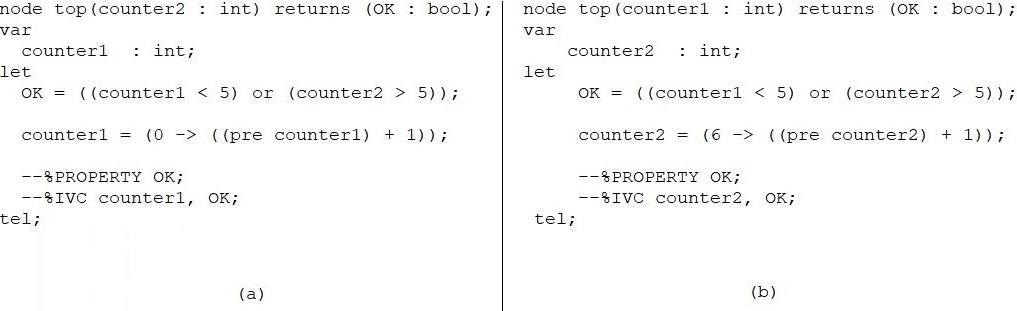
\includegraphics[width=\textwidth]{figs/absbvc.jpg}
  %\vspace{-0.1in}
  \caption{Building abstraction using BVCs}
  \vspace{0.1in}
  \label{fig:absbvc}
  \vspace{0.1in}
\end{figure}


Another observation is that if we calculate \emph{all} BVCs at a given depth for a valid property, there should be at least one BVC, which is the subset of one of the MIVCs. As we advance towards deeper bounds when BVCs stay the same, one may even conclude that BVC has already converged to an actual minimal IVC. However, this conclusion is not always accurate. It is possible that final MIVC is a superset of multiple BVCs at different bounds. Consider the toy example in Figure \ref{fig:toybvc}. If the initial value of {\small{\texttt{counter2}}} changes from 6 to 3, the MIVC of the property will be {\small{\texttt{\{counter1, counter2, OK\}}}} because the correctness of {\small{\texttt{OK}}} is dependent on both counters. However, if we obtain the BVCs for this new model (Figure \ref{fig:toybvc2}), you will see that BVC up to depth 5 is  {\small{\texttt{\{counter1, OK\}}}}, thereafter becomes {\small{\texttt{\{counter2, OK\}}}} and will not change (Figure \ref{fig:toyo2}).

\begin{figure}
 \centering
  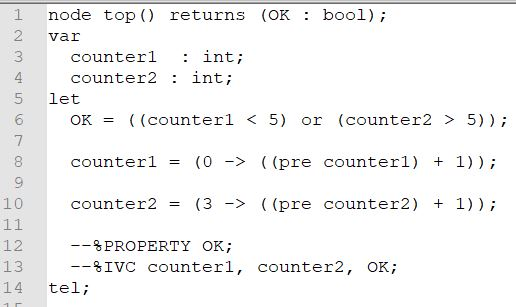
\includegraphics[width=0.70\columnwidth]{figs/toybvc2.jpg}
  %\vspace{-0.1in}
  \caption{A toy example where MIVC is the superset of multiple unique BVCs}
  \vspace{0.1in}
  \label{fig:toybvc2}
\end{figure}

\begin{figure}
 \centering
  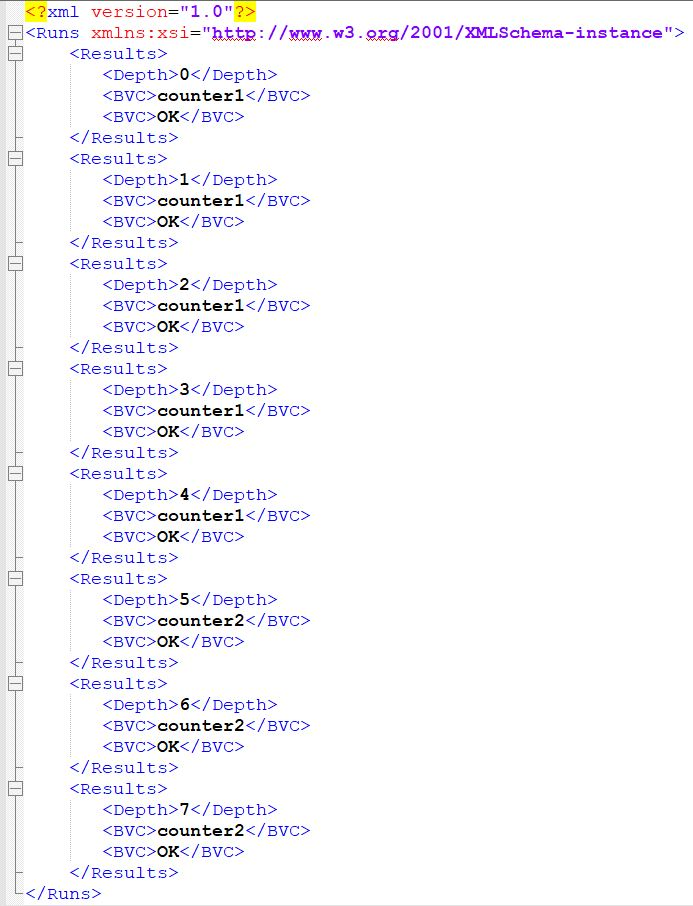
\includegraphics[width=0.8\columnwidth]{figs/toyo2.jpg}
  %\vspace{-0.1in}
  \caption{BVCs for the property in Figure \ref{fig:toybvc2}}
  \vspace{0.1in}
  \label{fig:toyo2}
\end{figure} 
